\section{Comparación de clasificadores e integradores}
\label{sec:correcciones-noviembre}

La clasificación de una trayectoria depende de la ventana observada y de la
discretización. Comparamos estos efectos mediante los sondeos de Chua
entero, dos integradores de Caputo de memoria completa, bancos de exponentes
y generadores de semillas en PLL y MAVPD. En cada comparación mantenemos
fijos los parámetros del campo y distinguimos las operaciones que cambian.

\subsection{Una visita próxima al equilibrio no determina el destino}

Una trayectoria puede permanecer cerca de un equilibrio inestable durante
un intervalo largo y abandonarlo después. El ejemplo escalar
\(\dot u=\lambda u\), \(\lambda>0\), permite verlo sin aproximaciones:
\[
 u(t)=u_0e^{\lambda t},\qquad
 |u(t)|<\varepsilon
 \quad\Longleftrightarrow\quad
 t<\frac1\lambda\log\frac{\varepsilon}{|u_0|}.
\]
Para cualquier ventana \(W>0\), basta elegir
\(0<|u_0|<\varepsilon e^{-\lambda W}\) para que toda esa ventana permanezca
cerca del origen, aunque \(|u(t)|\) crezca después. Así, una visita prolongada
no basta para asignar un destino de equilibrio.

En el control de Chua entero con 2001 muestras, la regla de detención
temprana asigna equilibrio durante una visita inicial; la trayectoria
completa alcanza después la norma 80 en \(t=7.11\). La regla terminal
observa el horizonte completo o el primer evento de terminación. Para
asignar equilibrio, exige que las últimas muestras elegibles permanezcan
próximas al mismo punto. Las visitas previas, las ventanas insuficientes,
los cruces de norma y los fallos numéricos se distinguen como desenlaces
de diferente significado.

Integramos un conjunto independiente de 504 condiciones iniciales,
con muestreo uniforme en volumen en bolas: tres equilibrios, siete radios
entre $10^{-5}$ y $10^{-2}$ y 24 puntos por combinación. Se fijaron antes
del cálculo el generador PCG64, la semilla 20261109, $q=1$, $h=.01$,
$T=320$, descarte 80, tolerancia de equilibrio .03, ventana de 90
muestras y norma umbral 80. Ambas políticas se evaluaron sobre las mismas
trayectorias. Las direcciones de este conjunto se generan con PCG64 y
son independientes de las del banco EFORK--3.

\begin{center}
\begin{tabular}{lrr}
\toprule
Desenlace & Regla temprana & Regla terminal\\\midrule
Equilibrio & 458 & 168\\
Cruce de norma & 27 & 171\\
Inconcluso & 19 & 165\\\bottomrule
\end{tabular}
\end{center}

De las capturas tempranas, 144 cruzan después el umbral y 146 no satisfacen
la condición terminal. Los 168 destinos de equilibrio corresponden al
origen. Tres controles inicializados exactamente en los equilibrios
permanecen estacionarios hasta 320. Cuatro PVI preseleccionados coinciden
en clase con DOP853; la mayor diferencia del tiempo de cruce es .007292,
inferior al paso .01. Estos cuatro controles no estiman una tasa poblacional
de error. La figura muestra bolas, no muestreo sobre superficies esféricas.

\begin{hafocommonfigure}[htbp]
\centering
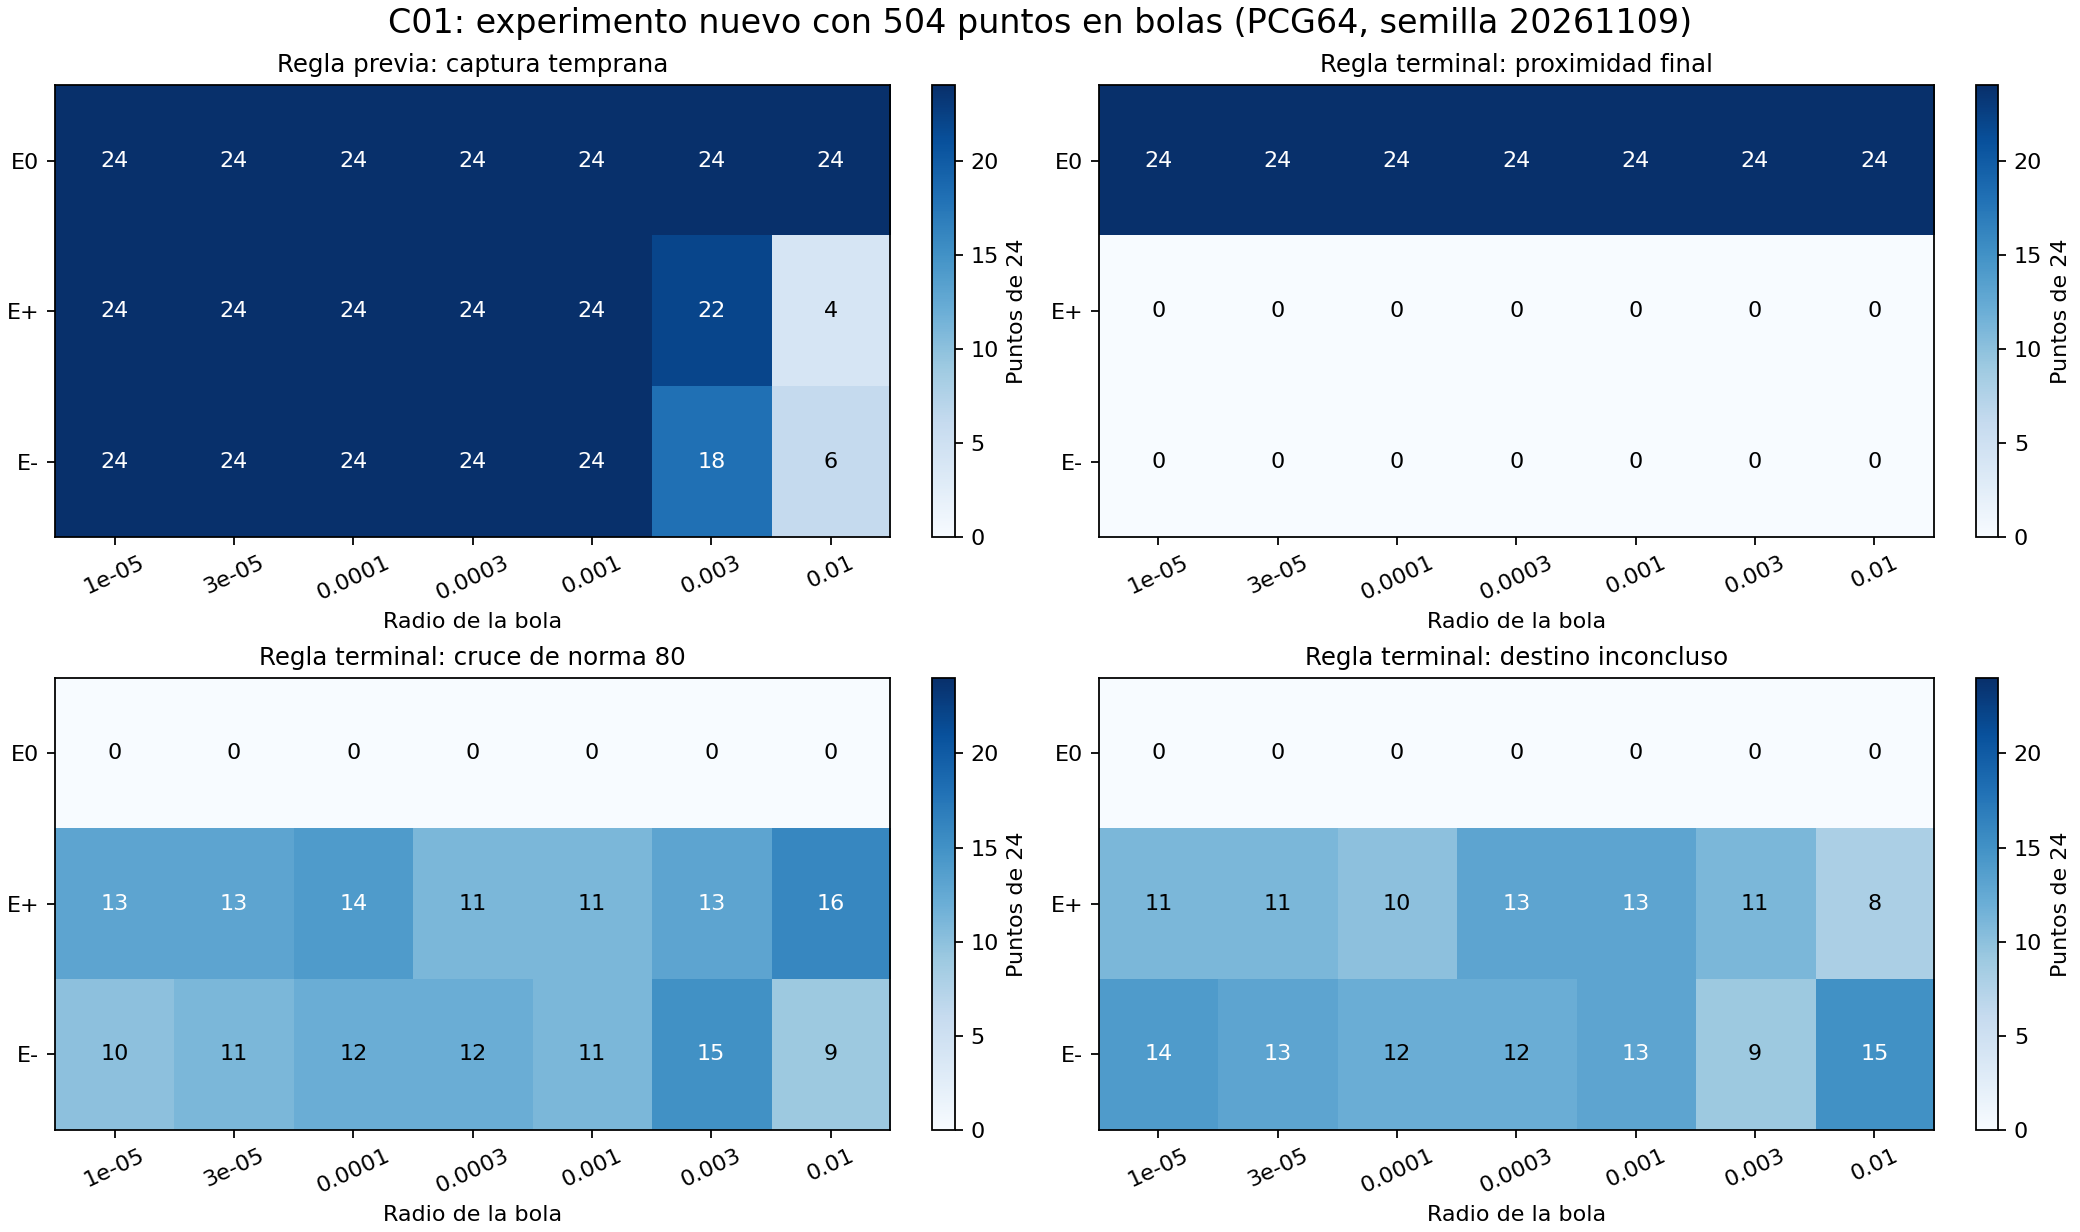
\includegraphics[width=.92\linewidth]{figures/correcciones/comparacion_504_politicas.png}
\caption{Chua entero: contraste de dos reglas sobre las mismas 504
trayectorias. El incremento de cruces registrados resulta de observar
la evolución posterior a visitas próximas al equilibrio.}
\end{hafocommonfigure}

\subsection{Sensibilidad de c590 al paso y al integrador}

Comparamos L1 implícito, resuelto con Newton y jacobiano analítico, con
PECE de pesos estables y suma compensada. Ambos conservan la historia desde
\(t_0=0\), pero aproximan objetos distintos: L1 discretiza la integral
que define la derivada de Caputo y PECE discretiza la ecuación de Volterra.

Para deducir L1 tomamos \(t_n=nh\), \(0<q<1\), y escribimos
\[
 {}^{\mathrm C}D_0^q x(t_n)
 =\frac1{\Gamma(1-q)}\sum_{k=0}^{n-1}
  \int_{t_k}^{t_{k+1}}(t_n-s)^{-q}x'(s)\,\dd s.
\]
En cada intervalo sustituimos \(x'(s)\) por la pendiente
\((x_{k+1}-x_k)/h\). La integral del núcleo es
\begin{align*}
 \int_{t_k}^{t_{k+1}}(t_n-s)^{-q}\,\dd s
 &=\frac{(t_n-t_k)^{1-q}-(t_n-t_{k+1})^{1-q}}{1-q}\\
 &=\frac{h^{1-q}}{1-q}
       [(n-k)^{1-q}-(n-k-1)^{1-q}].
\end{align*}
Multiplicamos por la pendiente y usamos
\((1-q)\Gamma(1-q)=\Gamma(2-q)\). Finalmente, el cambio de índice
\(j=n-k-1\) transforma la aproximación en
\begin{equation}
 \frac1{\Gamma(2-q)h^q}
 \sum_{j=0}^{n-1}b_j(x_{n-j}-x_{n-j-1})=F(x_n),
 \qquad b_j=(j+1)^{1-q}-j^{1-q}.
 \label{eq:comparacion-l1}
\end{equation}
El peso más reciente es \(b_0=1\). Si
\(c_q=\Gamma(2-q)h^q\) y
\(H_n=\sum_{j=1}^{n-1}b_j(x_{n-j}-x_{n-j-1})\), la incógnita satisface
\[
 R_n(x)=x-x_{n-1}+H_n-c_qF(x)=0,\qquad
 DR_n(x)=I-c_qDF(x).
\]
En una iteración de Newton resolvemos
\[
 [I-c_qDF(x^{(m)})]\Delta x^{(m)}=-R_n(x^{(m)}),\qquad
 x^{(m+1)}=x^{(m)}+\Delta x^{(m)}.
\]
La historia \(H_n\) permanece fija durante esa resolución. La existencia
de una solución de cada paso y la convergencia de Newton dependen de la
regularidad del campo y de la invertibilidad del jacobiano de ese residual.

Al tomar \(q\to1^-\), cada \(b_j\) con \(j\geq1\) tiende a cero,
\(b_0=1\) y \(c_q\to h\). Por tanto,
\cref{eq:comparacion-l1} se reduce a
\(x_n-x_{n-1}=hF(x_n)\), el paso de Euler implícito. El amortiguamiento
de esta discretización a paso grueso puede modificar una captura; por eso
contrastamos ambos métodos a tres pasos en vez de elegir uno como
referencia absoluta. En los controles analíticos se usa un piso de error
de \(5\times10^{-14}\) al comparar refinamientos próximos al redondeo
de máquina.

Se fijaron $q=.9999$, $h=.005,.0025,.00125$, $T=180$, descarte 90,
terminal inferior cero, norma umbral 120 y la misma referencia de contacto.
Seis PVI diagnósticos y tres equilibrios dan 54 integraciones.
Los seis PVI se eligieron por su función diagnóstica: no representan una
muestra aleatoria de la cuenca. Hubo siete acuerdos de etiqueta entre
métodos en 18 comparaciones; cuatro de los seis PVI cambian alguna
etiqueta al variar método o paso. Las tres condiciones de equilibrio
conservan su clase en todos los ensayos. No hubo fallos de Newton y el
mayor defecto L1 recalculado de forma independiente fue
$1.615\times10^{-14}$.

La semilla de referencia con PECE y $h=.0025$ cruza la norma en $t=176.05$,
mientras los pasos vecinos tienen otros desenlaces finitos. Los signos de
contacto corresponden a una referencia y a su reflejo. Como ambas nubes
intervienen en la misma regla de distancia, un cambio de signo no identifica
por sí solo una respuesta asintótica distinta. Los cambios de destino con
el método o el paso muestran sensibilidad numérica; en estas condiciones el mapa
finito no determina una cuenca robusta respecto de la discretización ni una
respuesta acotada hasta $T=300$.

\subsection{Reproducción de espectros: criterio y protocolo}

La comparación de espectros considera simultáneamente la tolerancia
numérica y el patrón de signos. Al aplicar ese criterio a los 24 espectros
calculados con referencia arrastrada entre bloques, obtenemos siete acuerdos
cuantitativos, ocho acuerdos de signos y nueve discrepancias.
En este banco, acuerdo cuantitativo exige error absoluto menor que .05 en
los tres componentes y los signos requeridos. La categoría abreviada
``sólo signos'' exige además error del primer exponente menor que .15;
no significa que se haya omitido toda tolerancia.

El método de Fischer y colaboradores~\cite{fischer2020}, sección 2.2,
ecuaciones (10), (20) y (21), identifica una referencia independiente
precalculada y el anclaje de cada bloque de clones al estado de esa
referencia en el tiempo físico correspondiente. Transportar el extremo del bloque corto como nueva referencia cambia
ese anclaje. Además, en el sistema financiero se distinguen
$h_{\rm ref}=.05$ y $h_{\rm clone}=.01$; igualarlos cambia la
discretización de la trayectoria de referencia.

Se implementó la referencia PECE de memoria completa con almacenamiento
lineal y convoluciones por bloques FFT. Los bloques FFT conservan las
contribuciones de toda la historia; no son reinicios del PVI. Los clones
sí reinician su memoria según el estimador publicado, y el bloque
siguiente vuelve a anclarse a la referencia independiente. Por ello este
banco no demuestra que se hayan calculado exponentes globales del PVI
Caputo causal con historia fija. Los controles comparan todos los puntos
con sumas directas, órdenes heterogéneos y soluciones analíticas.

Calculamos las 24 configuraciones con una referencia independiente de
memoria completa.
Para Jerk, la sección 3.1 y la condición III de la tabla 2 del artículo
motivan $T_{\rm clone}=10$, $N_{\rm clone}=1000$, $K=100$ y permiten comparar esa duración con una ventana de una unidad.
Evaluamos las ocho configuraciones de órdenes de Jerk en ambas ventanas,
conservando las mismas tolerancias de comparación.

\begin{center}
\begin{tabular}{lrrr}
\toprule
Comparación de los 24 espectros & Cuantitativo & Sólo signos & Fallo\\\midrule
Referencia arrastrada entre bloques & 7 & 8 & 9\\
Referencia independiente, ventanas iniciales & 11 & 6 & 7\\
Referencia independiente y ventana diez en Jerk & 18 & 4 & 2\\\bottomrule
\end{tabular}
\end{center}

La última combinación usa las nuevas filas financieras y de cuatro alas,
y las ocho filas Jerk a ventana diez. Dos filas fallan: financiero con
órdenes $(.9,1,1)$ y Jerk con $(.7,1,1)$. Otras cuatro sólo reproducen el
signo. El acuerdo cuantitativo alcanza así 18 de las 24 configuraciones. En Rabinovich--Fabrikant
de Danca y Kuznetsov~\cite{DancaKuznetsov2018Lyapunov} se conserva el error
del tercer exponente, aproximadamente .2525353 frente a tolerancia .05.
Un diagnóstico de otro parámetro no justifica alterar el caso publicado.

\subsection{Ocho repeticiones y costo de las rutas de semillas}

Comparamos PLL y MAVPD mediante ocho repeticiones de doce semillas por
ruta. Se separan centros algebraicos y perturbaciones; las
realizaciones uniformes y las posiciones dentro de cada celda de las mallas
varían entre repeticiones. Se conservaron los dominios, horizontes y
parámetros del piloto, con RK4 y DOP853. Nueve rutas en total dan 864
semillas de candidatos y siete controles adicionales: 1742 integraciones.
Los 864 pares de candidatos y los siete pares de controles coinciden en
clase y destino operacional.

\begin{center}
\begin{tabular}{llcc}
\toprule
Sistema & Ruta & Contactos de 12: mediana & Mínimo--máximo\\\midrule
PLL & PP y entorno & 6 & 6--6\\
PLL & Uniforme & 5 & 4--7\\
PLL & $\det J=0$ & 5.5 & 4--6\\
PLL & Malla & 5 & 4--7\\
MAVPD exterior & PP y entorno & 0 & 0--0\\
MAVPD exterior & Función descriptiva & 6 & 6--6\\
MAVPD exterior & Uniforme & 10 & 7--12\\
MAVPD exterior & $\det J=0$ & 10.5 & 9--12\\
MAVPD exterior & Malla & 11 & 10--12\\\bottomrule
\end{tabular}
\end{center}

En MAVPD, PP obtiene 91 contactos interiores de 96 semillas y cinco
transitorios; la función descriptiva reparte 48 contactos exteriores y
48 interiores. Medir sólo el destino exterior ocultaría esta diferencia
de cobertura. La ruta PP es estable en PLL, pero su resultado no supera
todas las realizaciones uniformes. La comparación cubre estas dos configuraciones; para evaluar la
generalización a otras familias necesitamos sistemas adicionales.

Se midieron generación efectiva de fórmulas, raíces y Jacobianos,
integración, clasificación, almacenamiento y preparación. En MAVPD,
la mediana de generación es 1.834 ms para función descriptiva y .170 ms
para PP; en PLL, .203 ms para PP. Integrar domina el costo, pero estas
medidas no incluyen como trabajo en línea las derivaciones algebraicas
previas ni la selección del modelo. El reloj de CPU por hilo presenta
cuantización: una lectura cero en una generación corta significa menor
que su resolución, no costo nulo. Los tiempos de pared se midieron con
otros procesos activos y no se interpretan como rendimiento absoluto.

\begin{hafocommonfigure}[htbp]
\centering
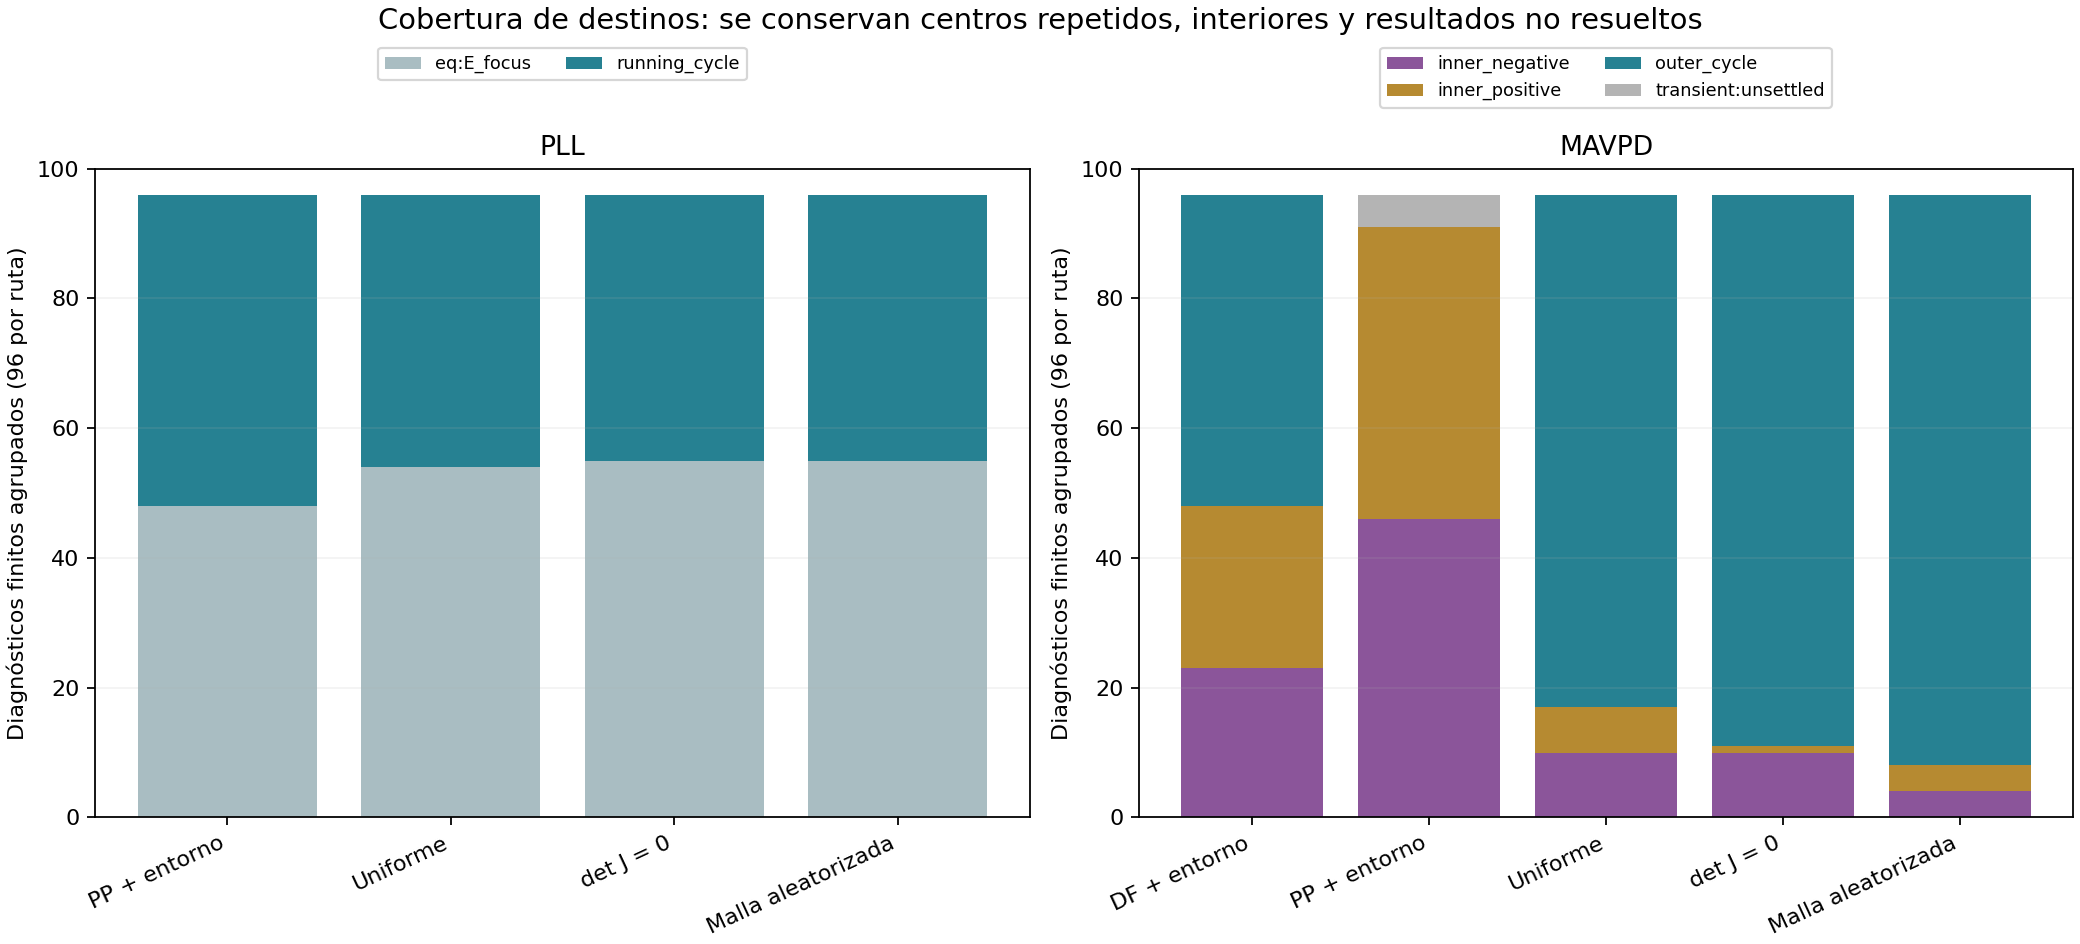
\includegraphics[width=.96\linewidth]{figures/correcciones/cobertura_multidestino.png}
\caption{Cobertura operacional de destinos en las ocho repeticiones.
La referencia exterior no agota las respuestas de interés de MAVPD.
Se muestran resultados finitos, sin convertir contacto en identidad
asintótica de atractores.}
\end{hafocommonfigure}

\subsection{Lorenz generalizado: un control de la propuesta FPP--A}

Se integró el campo
\[
 F(x,y,z)=(-3.4x+3.4y+.5yz,\;6.8x-y-xz,\;-z+xy)
\]
con $q=.995$, $T=60$, descarte 30 y los mismos tres pasos y dos métodos
del contraste independiente. Se fijaron dos FPP--A impresos, dos
perturbaciones simétricas del uno por ciento, dos iniciales uniformes y
tres equilibrios: 54 integraciones nuevas. El cálculo algebraico proporciona los equilibrios,
el jacobiano y las condiciones FPP--A. Las coordenadas FPP--A redondeadas a binary64 tienen
$\|JF\|\simeq1.42128\times10^{-13}$, distinto del residuo de la
reconstrucción multiprecisión de la sección anterior.

Los dos FPP--A terminan próximos a los equilibrios simétricos en los seis
ensayos de cada semilla. Sus perturbaciones se aproximan a los mismos
equilibrios, pero PECE no satisface la condición predeclarada de amplitud
de la ventana terminal: amplitud aproximada 1.195--1.198 frente al límite
uno, aunque su distancia final es .107--.109. L1 satisface ese criterio.
Es una diferencia de transitorio y clasificación finita, no evidencia de
atractores distintos. Siete de nueve PVI mantienen sus seis etiquetas,
incluidos los tres controles de equilibrio. No hubo cruce de norma ni
fallos de Newton; la simetría calculada fue exacta a la precisión almacenada.
El resultado es un control negativo útil: la condición algebraica FPP--A
no garantiza el destino buscado.

\subsection{Destinos finitos en mapas del ADM local}

El ADM local de Wu y las discretizaciones de Caputo de historia completa
corresponden a evoluciones diferentes. En el primero, cada subintervalo
comienza con el valor puntual del anterior. En L1 y PECE, cada paso combina
contribuciones desde el terminal inferior. Para \(N\) pasos, la suma directa
de historia procesa
\[
 1+2+\cdots+N=\frac{N(N+1)}2
\]
contribuciones, de donde resulta el costo \(O(N^2)\). El almacenamiento
de estados y valores del campo crece como \(O(N)\).

En los mapas distinguimos equilibrio terminal, contacto con una referencia,
otra respuesta finita, cruce de norma, fallo numérico e inconcluso. La
ventana terminal permite separar la proximidad final a un equilibrio de
una visita transitoria. Los sondeos sobre superficies esféricas y los
sondeos uniformes en volumen responden a distribuciones distintas y se
analizan por separado.

Calculamos con ADM local tres mapas de $9\times9$
en los planos $xy$, $xz$ e $yz$: 243 celdas y 217 condiciones iniciales
únicas, con $q=.99$, $h=.01$ y $T=100$. Las 243 trayectorias alcanzaron
el horizonte. Se obtuvieron 120 etiquetas de media positiva, 120 de media
negativa y tres inicializaciones repetidas en el origen. El signo de una
media en una ventana finita no identifica un atractor ni demuestra caos
u ocultedad. Estas regiones de destino describen la evolución del ADM local en el
horizonte considerado. Su comparación con Caputo requiere integrar las
mismas condiciones mediante un método de memoria completa.
